% !TEX root = ../thesis.tex
% !TEX spellcheck = en-US

%% Leave first page empty
\thispagestyle{empty}

% - what (problem statement)
% - why (need statement)
% - how (approach)
% - related
% - results

\section{Introduction}

Language is one of the most complex behaviors our species has developed. We humans use it to efficiently transport knowledge between individuals and communicate even the most abstract concepts with it. It takes children years to learn to learn express their thoughts and the subtle nuances of one's language give a glimpse one's cultural environment and upbringing, one's emotional state and one's intellect.

Not surprisingly in the field of \gls{AI} and especially \gls{ML} building computer systems with linguistic capabilities and solving language-based problems poses one of the hardest challenges and has motivated decades of research in Computational Linguistics. In fact many of the famous test for universal machine intelligence are based on linguistic capabilities, among them the famous \emph{Turing test} by~\cite{Turing:1950aa} where the task is for a human judge to determine whether he is having a conversation with a human or a machine in order to determine if the machine can be called intelligent, or the \emph{compression test} proposed by~\cite{Mahoney:1999aa}, where a human's and machine's capability to predict missing words given a context is tested.

This thesis explores the specific task of predicting the semantic structure of job advertisements as a specific example of such a language-based task that turns out to be difficult even for humans to do. The title of this work ``An \emph{Exploration} of \emph{Recent Connectionist Advances} for \emph{Supervised Topic Prediction in Job Advertisements}'' can be broken down into three pieces that captures the essence of it:

\begin{itemize}
  \item Exploration: The nature of this work is explorative in 2 ways: First a problem has been researched to find well-defined and well-motivated application of machine learning on job advertisement data. Second a solution space was explored approach this problem with special emphasis at recent progress in research.
  \item Recent Connectionist Advances: The work
\end{itemize}


The work was done in close collaboration with the Helsinki-based media and learning company \emph{Sanoma}\footnote{\textquote{Sanoma is a front running consumer media and learning company in Europe. In Finland and the Netherlands we are the market leading media company with a broad presence across multiple platforms. In Belgium we are among the Top 5. Our main markets in learning are Belgium, Finland, the Netherlands, Poland and Sweden. We entertain, inform, educate and inspire millions of people every day. We employ some 7,500 professional employees operating in Europe.}, Source: \url{http://www.sanoma.com/en/who-we-are}, visited 06.06.2016} and the research motivation was thus constantly tied back into real world challenges in the scope of Sanoma's business needs.

\subsection{Problem Statement}

The problem addressed during with this thesis to better understand the structure of job advertisements. In particular job postings typically consist of several parts with a certain function or theme: Usually the company is introduced, the job is described with it's tasks and responsibilities, the requirements for the job are listed, then benefits and offerings by the company are named and the reader is asked to apply in a specified way he or she is interested.
Almost all of the text\footnote{Only 4\% of the sentences collected for evaluating the final experiments in this thesis were sorted into the category \emph{other} while the rest falls into either of the categories described. This is described in more detail in Section }\todo{link section} of a job description falls into these categories and the task can thus be posed as predicting a category for each sentence in a job advertisement, that corresponds with this sentence belonging to one of the job ads' parts as described above.
This is a challenging problem in itself but can further be used to extract certain functional parts of each job ad, to study a possible correlation between structural patterns and the reach and success of an ad and so forth. The problem therefore can be labelled as \emph{Text Categorization} or \emph{Text Classification} as referred to in the scientific literature.


\subsection{Motivation}

% -- need statement

Today's media and education, the basis of Sanoma's core businesses, are undergoing drastic and fundamental transformations that are currently disrupting whole industries.

Usage of digital media as a source of information has long surpassed print media. Sanoma's most well-known product, Finland's biggest daily newspaper \emph{Helsingin Sanomat}, lost 6\% of its circulation only in 2015\footnote{Source: http://www.digitalnewsreport.org/survey/2016/finland-2016/, visited 27.07.2016}, while the wide-spread use of social media challenges traditional ways we access information. Similarly in the field of education, with the rise of Massive open online course (MOOCs), traditional learning settings are challenged and the need for advanced techniques for data processing and analysis increases, e.g.\ to personalize and adapt the learning experience to each individual user and at the same time identify trends across large groups of learners to better meet the needs of education.

Sanoma provides a recruitment platform named \emph{Oikotie Työpaikat}. The service is in direct competition several other international players in the recruitment industry. Through this and other services Sanoma's collects large amounts of user-generated data, offering the potential to be leveraged for machine learning solutions to provide value for their users and innovate and enrich the company's offerings.
This was the company's initial motivation for this thesis project --- To explore ways to leverage user-generated data to potentially.

% -- research motivation

% -- personal motivation

From a personal perspective this work was interesting as offered many research possibilities while at the same time being relevant for a real business. Natural Language Processing and Computer Linguistics had always been of strong interest to me for the complex nature and yet high interpretability of problems and their proximity and relatedness to progress in universal machine intelligence. This presented me with the challenge position to balance pursuing research objectives and yet exploring potential business and user needs, learn on new fronts and deepen my knowledge in others as well as combining my experience in Product Development and Innovation, thus made for a great project to mark the competition of my studies as a Master's student.

\subsection{Related work}
\label{sub:Related work}

The problem of \gls{TC}, also known as Text Categorization, is one of the various challenges in the thriving fields of \gls{CL} and \gls{NLP}. These areas of research have started out as theoretically challenging but rather marginally interesting fields between \gls{AI} and formal linguistics and have since exploded in terms of popularity with their applications being deployed currently at large scale to practically all kinds of consumer products such as smart phones and home entertainment systems as well as digital services like social networks or automatic translation engines and conversational agents, so-called chatbots.
Today there are textbooks dedicated specifically to this area, such as~\cite{Manning:1999aa},~\cite{Jurafsky:2014aa} and~\cite{Clark:2013aa} There is also much overlap to the field of \gls{IR} that rose to popularity during the late 1980's due to the Internet starting to become a mainstream medium (see~\cite{Manning:2008aa},~\cite{Leskovec:2014aa} and the classic work by~\cite{Rijsbergen:1979aa}).

The field of Natural Language Processing has undergone different trends of modeling approaches to tackle its challenges. \cite{Cambria:2014aa} identify these as three main trend curves focusing on \emph{Syntactics}, \emph{Semantics}, and \emph{Pragmatics}. According to the authors the first trend of syntax-centered NLP is still prevalent and is based on algorithms that more or less directly operate on the words found in the processed texts.
The second trend operates on the semantics of text, thus being able to potentially tackle more challenging problems by addressing increasingly subtle notions of meaning and context. According to the author these types of approaches are still in the early phase but at the verge of being adapted by a broader audience of researchers and practitioners in the field.
The last trend curve of pragmatics regards the yet more complex issue of modeling inherent narratives in language where so far only pioneering work has been done but which, according to the authors, will lead to tackling problems of natural language understanding.
% With regards to this perspective, this thesis falls between the first and second trend curve by comparing more traditional, syntax based approaches to those modeling latent semantics.

The problem of \gls{TC} specifically has seen many evolving fashions of approaches and more or less loosely follows the three trend curves described above. \gls{TC} has been of immense interest for several decades now due to the exponentially increasing amounts of text data being recorded in forms of e.g. user generated content through social networks and through the increased digitalization of our daily lives. Its applications reach from document filtering, automated metadata generation such as language classification to automatic email labeling, spam identification and sentiment detection, amongst others.

As~\cite{Sebastiani:2002aa} points out it is important to mention that the term \emph{automatic text classification} has also been used referring to different problems: \textquote{Aside from (i) the automatic assignment of documents to a predefined set of categories [\ldots], the term has also been used to mean (ii) the automatic identification of such a set of categories (e.g.,~\cite{Borko:1963aa}), or (iii) the automatic identification of such a set of categories and the grouping of documents under them (e.g.,~\cite{Merkl:1998aa}), a task usually called text clustering, or (iv) any activity of placing text items into groups, a task that has thus both TC and text clustering as particular instances~\cite{Manning:1999aa}}~\cite{Sebastiani:2002aa}

Early approaches towards solving text classification tasks in the 1980's were in often based on expert systems consisting of sets of manually created logical rules, deciding upon the category of a text segment if a certain formula applies. As discussed by \cite{Sebastiani:2002aa} the biggest downside is known as the \emph{knowledge acquisition bottleneck} which refers to the fact that each rule has to be manually created. In the 1980's machine learning approaches became more common where a \emph{classifier} automatically learns the attributes of the data and its association with the given data labels using a model that allows to then infer the categories for unseen data. This setting is called \emph{supervised learning} as labels for the data are given and predicted.

Machine learning approaches have since been developed in countless variations. As described earlier syntax-based approaches are still very common and most follow a classic pipeline of \emph{feature extraction} or \emph{indexing} of documents followed by \emph{inductive construction} of a classifier that is lastly evaluated by a measure of effectiveness. A very successful approach to feature extraction has been the introduction of N-Gram based models, also called \emph{bag-of-words} models, which that are based on word-cooccurrence frequencies of the terms that are present in the data.
As~\cite{Mikolov:2012aa} explains \textquote{The most significant advantages of models based on n-gram statistics are speed (probabilities of n-grams are stored in precomputed tables), reliability coming from simplicity, and generality (models can be applied to any domain or language effortlessly, as long as there exists some training data). N-gram models are today still considered as state of the art not because there are no better techniques, but because those better techniques are computationally much more complex, and provide just marginal improvements, not critical for success of given application.}
Various extensions of these models exist for dimensionality reduction or feature selection as well as smoothing techniques etc. (refer to Section~\ref{subs:N-gram Models} for an in-depth introduction). The limitation of such models is that their statistics are directly based on word co-occurrences and thus exponentially increase in size as the desired context to be captured is expanded, making them infeasible to adapt to longer text sequences.

Recently approaches from the field of \emph{Representation Learning}, have found their way into and gained tremendous traction in the \gls{NLP} research community. Traditional \emph{feature engineering} techniques such as N-gram models, use prior domain or expert knowledge in order to build data representations that are effective in combination with a classifier. But as~\cite{Bengio:2013aa} point out this is a laborious and time-consuming task that only exposes the weakness from a Machine Learning point of view by not automatically learning such representations --- a challenge representation learning aims to address.


- distributed representations beating ngrams
- deep learning: CNNs
- multitask / transfer learning
- character level text classification
% # CNNs
% \cite{Kim:2014aa} - Convolutional neural networks for sentence classification
% \cite{Cheng:2014aa} - Investigating the role of prior disambiguation in deep-learning compositional models of meaning
% \cite{Kalchbrenner:2014aa} - A convolutional neural network for modelling sentences
% \cite{Johnson:2014aa} - Effective Use of Word Order for Text Categorization with Convolutional Neural Networks


% ## related fields
%
% # NER
% \cite{Baluja:2000aa} - Applying Machine Learning for High-Performance Named-Entity Extraction
% \cite{Zhang:2004aa} - Zhang-Focused Named Entity Recognition Using
% \cite{Strzalkowski:1996aa} - A Self-learning Universal Concept Spotter
% \cite{Alfonseca:2002aa} - An unsupervised method for general named entity recognition and automated concept discovery
% \cite{Nadeau:2007aa} - A survey of named entity recognition and classification.
%
% # Topic modeling
% \cite{Blei:2012aa} - Probabilistic Topic Models
%
%
% # Ngram models
% \cite{Jagadish:1998aa} - Optimal histograms with quality guarantees
%
% # language modeling
% \cite{Bengio:2006aa} - Neural Probabilistic Language Models.
% \cite{Mikolov:2013aa} - Exploiting similarities among languages for machine translation.
% \cite{Mikolov:2012aa} - Statistical Language Models Based on Neural Networks
%
%
%
% # CNNs
% \cite{Kim:2014aa} - Convolutional neural networks for sentence classification
% \cite{Cheng:2014aa} - Investigating the role of prior disambiguation in deep-learning compositional models of meaning
% \cite{Kalchbrenner:2014aa} - A convolutional neural network for modelling sentences
% \cite{Johnson:2014aa} - Effective Use of Word Order for Text Categorization with Convolutional Neural Networks
%
%
%
% # sequential modeling
% \cite{Lafferty:2001aa} - Conditional Random Fields: Probabilistic Models for Segmenting and Labeling Sequence Data
%
% # \cite{Lewis:1992aa} - Feature selection and feature extraction for text categorization
%
%
% Unsupervised techniques for topic discovery have been investigated widely, such as LSA
%
% Vector Space models are a
%
% - feature learning for text
% - multitask learning
%
% \cite{Bastian:2014aa} - ontology learning, topic extraction approach
%
%
% \cite{Collobert:2008aa} showed how both multitask learning and semi-supervised learning improve the generalization of the shared tasks on text data. They describe \textquote{a single convolutional neural network architecture that, given a sentence, outputs [\ldots] part-of-speech tags, chunks, named entity tags, semantic roles, semantically similar words and the likelihood that the sentence makes sense (grammatically and semantically) using a language model}.
%
% \cite{Lodhi:2002aa} string kernels
%
% \todo{section on transfer learning and feature learning}
% \todo{text classification}
% \todo{Multitask learning}
% \todo{explicit vs implicit feature representation}


\subsection{Research Scope and Objectives}
\label{sub:Research Scope and Objectives}

This thesis was initiated as a research project for Sanoma's recruitment platform \emph{Oikotie Työpaikat} with the intention of exploring interesting and novel ways to use the various data generated through the use of this service. The research objectives were stated as follows:

\blockquote{Find an application of data mining / machine learning to the customer-generated data on the recruitment platform Oikotie Työpaikat which has the potential of bringing value to the user of the platform and is technically feasible in the scope of a master’s thesis. Further define and investigate a research problem that is essential to this application by researching literature and previous work on similar problems trying different approaches based on the literature using the results and learnings to create an improved approach.}

\todo{write this out}
on the research side
- define a good topic and scope
- evaluate solutions to that problem scope to find the best possible way of solving it, i.e. try cutting edge methods
- try to possibly built on ideas to adapt these methods for the problem to make them more effective or advance certain ideas

\subsection{Methodological Approach}
\label{sub:Methodological Approach}

\begin{figure}[h]
    \centering
    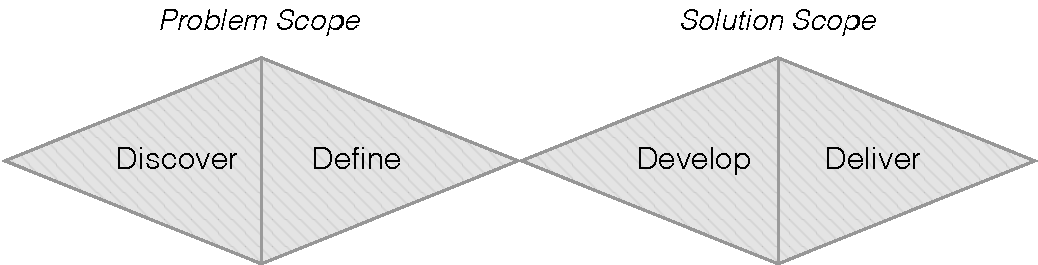
\includegraphics[width=\textwidth]{img/double-diamond.pdf}
    \caption{Design process for this thesis, adapted from the \emph{Double Diamond Process} developed by the British Design Council (see~\cite{Council:2007aa})}
\label{fig:double-diamond}
\end{figure}

The design and development process of the project was adapted from the double diamond approach that was developed by the by the British Design Council in 2005 (see ~\cite{Council:2007aa}). A design process is \textquote{the specific series of events, actions or methods by which a procedure or set of procedures are followed, in order to achieve an intended purpose, goal or outcome.}~\cite{Best:2006aa}.

\paragraph{Discover}
\label{par:Discover}

In the first stage of the project an initial idea, motivation or inspiration is given.

- prototyping
- interviews
- market research
-

approach to experiemtns



\subsection{Results}

asdasd

\subsection{Structure of the Thesis}

\begin{figure}[h]
    \centering
    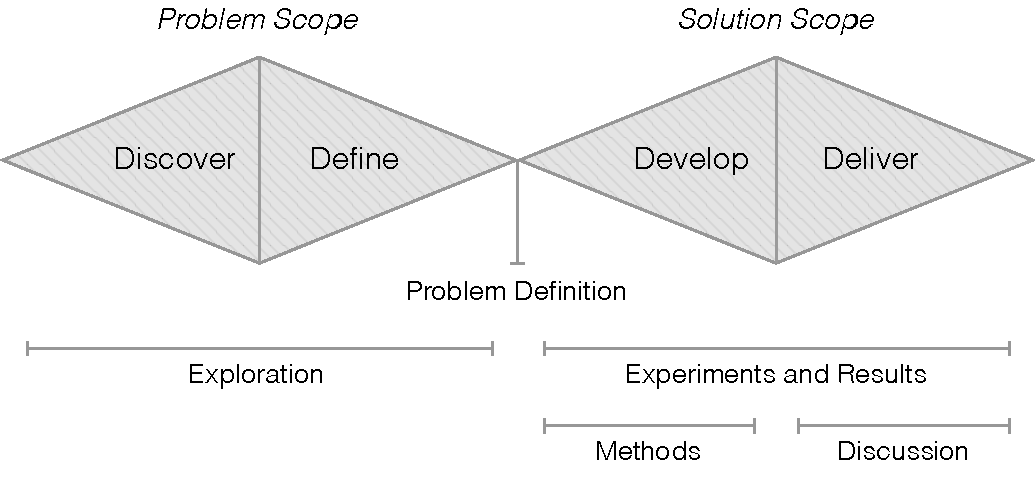
\includegraphics[width=\textwidth]{img/double-diamond-with-structure}
    \caption{Structure of this thesis mapped to the \emph{Double Diamond Process} design process }
\label{fig:double-diamond-with-structure}
\end{figure}

% The first section of this thesis gave a brief introduction into the topic of this work, outlined the motivation and the research problem approached and showed the research objectives, the scope of the thesis as well as related work.
%
% Section~\ref{sec:Background}:~\nameref{sec:Background} introduces the reader to concepts and ideas of Text Classification in order to provide him or her with the necessary knowledge to understand the work described in this thesis. First the problem of Text Classification is formally defined and the most common approaches to this problem are described on a high level. Afterwards Vector Space Models are introduced in detail, which represent a popular way of tackling this task by transforming text into fixed-size vectors.
% The following subsection then briefly presents several of the most known classification algorithms that can operate on the vectors produced by such Vector Space Models. Next the approach of Sequential Classification is described in short where text is treaded as a one-dimensional signal in time. The following subsection then shows common ways to evaluate how well the task of text classification is solved and the last subsection gives a brief introduction to two methods that are useful for exploring different models and techniques through visualization.
%
% Section~\ref{sec:Exploration}:~\nameref{sec:Exploration} gives an overview of the exploration of the wider topic space at the start of the thesis project as well as the experimentation with different techniques and the data given for the project. It aims to lay out to the reader the process, insights and learnings leading towards the final problem formulation and evaluation of methods to solve this problem.
%
% The following Section~\ref{sec:Experimental Evaluation of Multi-class Prediction of Semantic Categories for Text in Job Advertisements}:~\nameref{sec:Experimental Evaluation of Multi-class Prediction of Semantic Categories for Text in Job Advertisements} then presents the main results of the thesis. The exact problem definition is given that is used as a basis to evaluate the experiments and the dataset used for these experiments is described.
% Subsequently the evaluation of the different approaches to Vector Space Models, the classification algorithms using the most successful of these models and the sequential modeling approach are documented. Each of these subsections first describes the experimental setup, followed by results of the different approaches and closes with a brief discussion on the outcomes presented.
